\section{Existence and Uniqueness of Solutions}\label{sec:existence}

\asyouread{
%\item Can a system of two equations and two unknowns have no solution?
\item T/F: It is possible for a linear system to have exactly 5 solutions.
\item T/F: A variable that corresponds to a leading 1 is ``free.''
\item	How can one tell what kind of solution a linear system of equations has?
\item	Give an example (different from those given in the text) of a 2 equation, 2 unknown linear system that is not consistent.
%\item T/F: If a linear system implies that $0=1$, then it has no solution.
\item T/F: A particular solution for a linear system with infinite solutions can be found by arbitrarily picking values for the free variables.
}

So far, whenever we have solved a system of linear equations, we have always found exactly one solution. This is not always the case; we will find in this section that some systems do not have a solution, and others have more than one. 

%So far, all of the examples of systems of linear equations that we have seen have had a solution; in fact, there has always been exactly one solution. We hinted at the end of the last section that this will not always be the case. In this section we explore the different possibilities and how we can recognize when they arise.

We start with a very simple example. Consider the following linear system: $$x-y=0.$$ There are obviously infinite solutions to this system; as long as $x=y$, we have a solution. We can picture all of these solutions by thinking of the graph of the equation $y=x$ on the traditional $x,y$ coordinate plane.

Let's continue this visual aspect of considering solutions to linear systems. Consider the system \begin{align*} x+y&=2\\ x-y&=0. \end{align*} Each of these equations can be viewed as lines in the coordinate plane, and since their slopes are different, we know they will intersect somewhere (see Figure \ref{fig:visual_solution} (a)). In this example, they intersect at the point $(1,1)$ -- that is, when $x=1$ and $y=1$, both equations are satisfied and we have a solution to our linear system. Since this is the only place the two lines intersect, this is the only solution. 

Now consider the linear system \begin{align*} x+y&=1\\2x+2y&=2.\end{align*} It is clear that while we have two equations, they are essentially the same equation; the second is just a multiple of the first. Therefore, when we graph the two equations, we are graphing the same line twice (see Figure \ref{fig:visual_solution} (b); the thicker line is used to represent drawing the line twice). In this case, we have an infinite solution set, just as if we only had the one equation $x+y=1$. We often write the solution as $x=1-y$ to demonstrate that $y$ can be any real number, and $x$ is determined once we pick a value for $y$. 

%\begin{figure}\begin{center}\includegraphics[width=.25\linewidth]{MA_103_MetaPost_Figures/01_Existence_Intersect}$\quad$\includegraphics[width=.25\linewidth]{MA_103_MetaPost_Figures/01_Existence_Nonunique}$\quad$\includegraphics[width=.25\linewidth]{MA_103_MetaPost_Figures/01_Existence_Inconsistent}\caption{The three possibilities for two linear equations with two unknowns.} \label{fig:visual_solution}\end{center}\end{figure}

\begin{myfigure}\begin{center}
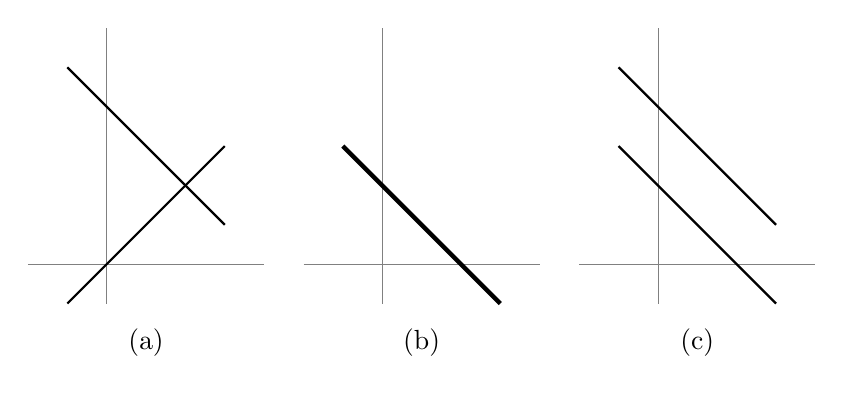
\begin{tikzpicture}

\draw[gray, very thin] (0,-.5) -- (0,3);
\draw[gray, very thin] (-1,0) -- (2,0);
\draw [thick] (-.5,-.5) -- (1.5,1.5);
\draw [thick] (-.5,2.5) -- (1.5,.5);
\node at (.5,-1) {(a)};

\draw[gray, very thin] (3.5,-.5) -- (3.5,3);
\draw[gray, very thin] (2.5,0) -- (5.5,0);
\draw[ultra thick] (3,1.5) -- (5,-.5);
\node at (4,-1) {(b)};

\draw[gray, very thin] (7,-.5) -- (7,3);
\draw[gray, very thin] (6,0) -- (9,0);
\draw[thick]  (6.5,1.5) -- (8.5,-.5);
\draw[thick]  (6.5,2.5) -- (8.5,.5);
\node at (7.5,-1) {(c)};

\end{tikzpicture}
\mycaption{The three possibilities for two linear equations with two unknowns.} \label{fig:visual_solution}
\end{center}
\end{myfigure}

Finally, consider the linear system \begin{align*} x+y&=1\\x+y&=2.\end{align*} We should immediately spot a problem with this system; if the sum of $x$ and $y$ is 1, how can it also be 2? There is no solution to such a problem; this linear system has no solution. We can visualize this situation in Figure \ref{fig:visual_solution} (c); the two lines are parallel and never intersect.

If we were to consider a linear system with three equations and two unknowns, we could visualize the solution by graphing the corresponding three lines. We can picture that perhaps all three lines would meet at one point, giving exactly 1 solution; perhaps all three equations describe the same line, giving an infinite number of solutions; perhaps we have different lines, but they do not all meet at the same point, giving no solution. We further visualize similar situations with, say, 20 equations with two variables.

While it becomes harder to visualize when we add variables, no matter how many equations and variables we have, solutions to linear equations always come in one of three forms: exactly one solution, infinite solutions, or no solution. This is a fact that we will not prove here, but it deserves to be stated.

\theorem{thm:existence_uniqueness}{\textbf{Solution Forms of Linear Systems}\\

Every linear system of equations has exactly one solution, infinite solutions, or no solution.}\index{solution!types}\index{solution!unique} \index{solution!infinite}\index{solution!none}

This leads us to a definition. Here we don't differentiate between having one solution and infinite solutions, but rather just whether or not a solution exists.

\definition{def:consistent}{\textbf{Consistent and Inconsistent Linear Systems}\\

A system of linear equations is \textit{consistent} if it has a solution (perhaps more than one). A linear system is \textit{inconsistent} if it does not have a solution.}\index{system of linear equations!consistent} \index{system of linear equations!inconsistent} \index{consistent} \index{inconsistent}

How can we tell what kind of solution (if one exists) a given system of linear equations has? The answer to this question lies with properly understanding the reduced row echelon form of a matrix. To discover what the solution is to a linear system, we first put the matrix into reduced row echelon form and then interpret that form properly.

Before we start with a simple example, let us make a note about finding the \rref\ of a matrix.\\

\textsf{\textbf{ Technology Note:}} In the previous section, we learned how to find the \rref\ of a matrix using Gaussian elimination -- by hand. We need to know how to do this; understanding the process has benefits. However, actually executing the process by hand for every problem is not usually beneficial. In fact, with large systems, computing the \rref\ by hand is effectively impossible. Our main concern is \textit{what} ``the rref'' is, not what exact steps were used to arrive there.
%In the two previous examples, we found the \rref\ of a matrix and found the solution using this form. We did not, however, show the steps necessary to find ``the rref.'' This will be our standard practice from here on out.
%It is beneficial to know how to perform these steps, but it is not beneficial to do them every time; most often, we are not interested in the process of finding the \rref, but rather the end result. 
Therefore, the reader is encouraged to employ some form of technology to find the \rref. Computer programs such as \textit{Mathematica}, MATLAB, Maple, and Derive can be used;
many handheld calculators (such as Texas Instruments calculators) will perform these calculations very quickly. 

As a general rule, when we are learning a new technique, it is best to not use technology to aid us. This helps us learn not only the technique but some of its ``inner workings.'' We can then use technology once we have mastered the technique and are now learning how to use it to solve problems.

From here on out, in our examples, when we need the \rref\ of a matrix, we will not show the steps involved. Rather, we will give the initial matrix, then immediately give the \rref\ of the matrix. We trust that the reader can verify the accuracy of this form by both performing the necessary steps by hand or utilizing some technology to do it for them.\\

Our first example explores officially a quick example used in the introduction of this section.\\

\example{ex_ex_un_01}{Find the solution to the linear system $$\begin{array}{ccccc} x_1 & +& x_2 & = & 1\\ 2x_1 & + & 2x_2 & = &2\end{array} . $$}
{Create the corresponding augmented matrix, and then put the matrix into \rref. 

$$\bmx{ccc} 1&1&1\\2&2&2\emx \qquad \overrightarrow{\text{rref}} \qquad \bmx{ccc} 1&1&1\\0&0&0\emx $$

Now convert the reduced matrix back into equations. In this case, we only have one equation, $$x_1+x_2=1$$ or, equivalently, 
\begin{align*} x_1 &=1-x_2\\ x_2&\text{ is free}. \end{align*}

We have just introduced a new term, the word \textit{free}.\index{free variable}\index{variable!free} It is used to stress that idea that $x_2$ can take on \textit{any} value; we are ``free'' to choose any value for $x_2$. Once this value is chosen, the value of $x_1$ is determined. We have infinite choices for the value of $x_2$, so therefore we have infinite solutions.

For example, if we set $x_2 = 0$, then $x_1 = 1$; if we set $x_2 = 5$, then $x_1 = -4$. 
}\\

Let's try another example, one that uses more variables.\\

\example{ex_ex_un_1}{Find the solution to the linear system 
$$\begin{array}{ccccccc}
 & &x_2&-&x_3&=&3\\
x_1&  & &+&2x_3&=&2\\
 &&-3x_2&+&3x_3&=&-9\\
 \end{array}.$$}
{To find the solution, put the corresponding matrix into \rref.

$$\bmx{cccc} 0&1&-1&3\\ 1&0&2&2\\ 0&-3&3&-9\emx \qquad \overrightarrow{\text{rref}} \qquad \bmx{cccc}1&0&2&2\\ 0&1&-1&3\\ 0&0&0&0 \emx$$

Now convert this reduced matrix back into equations. We have 
\begin{align*} x_1 + 2x_3 &= 2 \\ x_2-x_3&=3 \end{align*} 
or, equivalently, 
\begin{align*} x_1 &= 2-2x_3 \\ x_2&=3+x_3\\x_3&\text{ is free.} \end{align*}

These two equations tell us that the values of $x_1$ and $x_2$ depend on what $x_3 $ is. As we saw before, there is no restriction on what $x_3$ must be; it is ``free'' to take on the value of any real number. Once $x_3$ is chosen, we have a solution. Since we have infinite choices for the value of $x_3$, we have infinite solutions. 

As examples, $x_1 = 2$, $x_2 = 3$, $x_3 = 0$ is one solution; $x_1 = -2$, $x_2 = 5$, $x_3 = 2$ is another solution. Try plugging these values back into the original equations to verify that these indeed are solutions. (By the way, since infinite solutions exist, this system of equations is consistent.)}\\ 
%\eexset

%%%
%%% Had issues around here with line spacing - new paragraphs also had vertical space in them. Not sure why ... could fix
%%% it with new pages, etc.
%%%

In the two previous examples we have used the word ``free'' to describe certain variables. What exactly is a free variable? How do we recognize which variables are free and which are not? 

Look back to the reduced matrix in Example \ref{ex_ex_un_01}. Notice that there is only one leading 1 in that matrix, and that leading 1 corresponded to the $x_1$ variable. That told us that $x_1$ was \textit{not} a free variable; since $x_2$ \textit{did not} correspond to a leading 1, it was a free variable.

Look also at the reduced matrix in Example \ref{ex_ex_un_1}. There were two leading 1s in that matrix; one corresponded to $x_1$ and the other to $x_2$. This meant that $x_1$ and $x_2$ were not free variables; since there was not a leading 1 that corresponded to $x_3$, it was a free variable. 

We formally define this and a few other terms in this following definition.

\definition{def:free}{{\bf Dependent and Independent Variables}\\

Consider the \rref\ of an augmented matrix of a linear system of equations. Then:\\

a variable that corresponds to a leading 1 is a \textit{basic}, or \textit{dependent}, variable, and\index{variable!dependent}\index{variable!basic}\index{basic variable}\\

a variable that does not correspond to a leading 1 is a \textit{free}, or \textit{independent}, variable\index{variable!independent}\index{variable!free}\index{free variable}.}

One can probably see that ``free'' and ``independent'' are relatively synonymous. It follows that if a variable is not independent, it must be dependent; the word ``basic'' comes from connections to other areas of mathematics that we won't explore here.

%%%%

%We now consider the cases where we have infinite solutions to a system of linear equations. What does the \rref\ of the corresponding augmented matrix look like?

%Since we know that we have a solution, we know that there isn't a leading 1 in the last column (since this implies no solution). If we have a leading 1 for each variable, then we would have only one solution, for each row of our reduced matrix would correspond to an equation like $x_1 = 4$; each variable would be assigned a specific value. Therefore, to have infinite solutions, we need to have more variables than leading 1s.

These definitions help us understand when a consistent system of linear equations will have infinite solutions. If there are no free variables, then there is exactly one solution; if there are any free variables, there are infinite solutions. 

\keyidea{idea:consistent}{{\bf Consistent Solution Types}\\

A consistent linear system of equations will have exactly one solution if and only if there is a leading 1 for each variable in the system. \index{system of linear equations!consistent} \index{leading one} \index{solution!infinite}  \\

If a consistent linear system of equations has a free variable, it has infinite solutions.\\

If a consistent linear system has more variables than leading 1s, then the system will have infinite solutions.\\

A consistent linear system with more variables than equations will always have infinite solutions.\index{system of linear equations!consistent}\index{leading one}\index{solution!infinite}}

\textsf{\textbf{Note:}} Key Idea \ref{idea:consistent} applies only to \textit{consistent} systems. If a system is \textit{inconsistent}, then no solution exists and talking about free and basic variables is meaningless.\\

When a consistent system has only one solution, each equation that comes from the \rref\ of the corresponding augmented matrix will contain exactly one variable. If the consistent system has infinite solutions, then there will be at least one equation coming from the \rref\ that contains more than one variable. The ``first'' variable will be the basic (or dependent) variable; all others will be free variables. 

We have now seen examples of consistent systems with exactly one solution and others with infinite solutions. How will we recognize that a system is inconsistent? Let's find out through an example.\\

%Now that we understand \textit{when} we have infinite solutions, the only remaining thing to discuss is how to properly write that situation in a meaningful way. 

%We know that when we have infinite solutions, we have more variables than leading 1s. The variables that do not correspond to leading 1s will be \textit{free}, or \textit{independent}, variables. We are ``free'' to choose any value for these variables; they do not ``depend'' on anything or any other variable. The variables that do correspond to leading 1s are \textit{dependent}  variables; they depend on the values of independent variables or the values of constants. Look back at Example \ref{ex:ex_un_1} and identify which variables are independent and which are dependent. Notice how the values of the dependent variables depend on the value of the independent variable.

%%%%


%Let's consider another example.

\example{ex_ex_un_2}{Find the solution to the linear system
$$\begin{array}{ccccccc}
x_1&+&x_2&+&x_3&=&1\\
x_1&+&2x_2&+&x_3&=&2\\
2x_1&+&3x_2&+&2x_3&=&0\\
\end{array}.$$}
{We start by putting the corresponding matrix into \rref.

$$\bmx{cccc} 1&1&1&1\\1&2&1&2\\ 2&3&2&0\\ \emx \qquad \overrightarrow{\text{rref}} \qquad \bmx{cccc} 1&0&1&0\\ 0&1&0&0\\ 0&0&0&1\\ \emx$$

Now let us take the reduced matrix and write out the corresponding equations. The first two rows give us the equations \begin{align*} x_1+x_3&=0\\ x_2 &= 0.\\ \end{align*} So far, so good. However the last row gives us the equation $$0x_1+0x_2+0x_3 = 1$$ or, more concisely, $0=1$. Obviously, this is not true; we have reached a contradiction. Therefore, no solution exists; this system is inconsistent.}\\  % \eexset

In previous sections we have only encountered linear systems with unique solutions (exactly one solution). Now we have seen three more examples with different solution types. The first two examples in this section had infinite solutions, and the third had no solution. How can we tell if a system is inconsistent?

A linear system will be inconsistent only when it implies that 0 equals 1. We can tell if a linear system implies this by putting its corresponding augmented matrix into \rref. If we have any row where all entries are 0 except for the entry in the last column, then the system implies 0=1. More succinctly, if we have a leading 1 in the last column of an augmented matrix, then the linear system has no solution. 

\keyidea{idea:inconsistent}{{\bf Inconsistent Systems of Linear Equations}\\

A system of linear equations is inconsistent if the \rref\ of its corresponding augmented matrix has a leading 1 in the last column.}\index{system of linear equations!inconsistent} \index{leading one}

\example{ex_ex_un_3}{Confirm that the linear system $$\begin{array}{ccccc} x&+&y&=&0 \\2x&+&2y&=&4 \end{array}$$ has no solution. }
{We can verify that this system has no solution in two ways. First, let's just think about it. If $x+y=0$, then it stands to reason, by multiplying both sides of this equation by 2, that $2x+2y = 0$. However, the second equation of our system says that $2x+2y= 4$. Since $0\neq 4$, we have a contradiction and hence our system has no solution. (We cannot possibly pick values for $x$ and $y$ so that $2x+2y$ equals both 0 and 4.)

Now let us confirm this using the prescribed technique from above. The \rref\  of the corresponding augmented matrix is $$\bmx{ccc} 1&1&0\\0&0&1\\ \emx.$$ We have a leading 1 in the last column, so therefore the system is inconsistent. }\\
%\eexset


%We now consider the cases where we have infinite solutions to a system of linear equations. What does the \rref\ of the corresponding augmented matrix look like?
%
%Since we know that we have a solution, we know that there isn't a leading 1 in the last column (since this implies no solution). If we have a leading 1 for each variable, then we would have only one solution, for each row of our reduced matrix would correspond to an equation like $x_1 = 4$; each variable would be assigned a specific value. Therefore, to have infinite solutions, we need to have more variables than leading 1s.

%\keyidea{idea:consistent}{A consistent linear system of equations will have exactly one solution if and only if there is a leading 1 for each variable in the system. \index{system of linear equations!consistent} \index{leading one} \index{solution!infinite}  \\
%
%If a consistent linear system has more variables than leading 1s, then the system will have infinite solutions.\\
%
%A consistent linear system with more variables than equations will always have infinite solutions.}\index{system of linear equations!consistent}\index{leading one}\index{solution!infinite}

%Now that we understand \textit{when} we have infinite solutions, the only remaining thing to discuss is how to properly write that situation in a meaningful way. 
%
%We know that when we have infinite solutions, we have more variables than leading 1s. The variables that do not correspond to leading 1s will be \textit{free}, or \textit{independent},\index{variable!independent} variables. We are ``free'' to choose any value for these variables; they do not ``depend'' on anything or any other variable. The variables that do correspond to leading 1s are \textit{dependent} \index{variable!dependent} variables; they depend on the values of independent variables or the values of constants. Look back at Example \ref{ex:ex_un_1} and identify which variables are independent and which are dependent. Notice how the values of the dependent variables depend on the value of the independent variable.
%
%More examples will help us.

Let's summarize what we have learned up to this point. Consider the \rref\ of the augmented matrix of a system of linear equations.\footnote{That sure seems like a mouthful in and of itself. However, it boils down to ``look at the reduced form of the usual matrix.''} If there is a leading 1 in the last column, the system has no solution. Otherwise, if there is a leading 1 for each variable, then there is exactly one solution; otherwise (i.e., there are free variables) there are infinite solutions.

Systems with exactly one solution or no solution are the easiest to deal with; systems with infinite solutions are a bit harder to deal with. Therefore, we'll do a little more practice. First, a definition: if there are infinite solutions, what do we call one of those infinite solutions?

\definition{def:particular}{\textbf{Particular Solution}\\ 

Consider a linear system of equations with infinite solutions. A \textit{particular solution} is one solution out of the infinite set of possible solutions.\index{particular solution}\index{solution!particular}}

The easiest way to find a particular solution is to pick values for the free variables which then determines the values of the dependent variables. Again, more practice is called for.\\



\example{ex_ex_un_4}{Give the solution to a linear system whose augmented matrix in \rref\ is $$\bmx{JJJJJ} 1&-1&0&2&4\\ 0&0&1&-3&7\\ 0&0&0&0&0\\ \emx$$ and give two particular solutions.}
{We can essentially ignore the third row; it does not divulge any information about the solution.\footnote{Then why include it? Rows of zeros sometimes appear ``unexpectedly'' in matrices after they have been put in \rref. When this happens, we do learn \textit{something}; it means that at least one equation was a combination of some of the others.} 
%We will learn more about this later.
 The first and second rows can be rewritten as the following equations: \begin{align*} x_1 - x_2 + 2x_4 &=4 \\ x_3 - 3x_4 &= 7. \\ \end{align*} Notice how the variables $x_1$ and $x_3$ correspond to the leading 1s of the given matrix. Therefore $x_1$ and $x_3$ are dependent variables; all other variables (in this case, $x_2$ and $x_4$) are free variables.

We generally write our solution with the dependent variables on the left and independent variables and constants on the right. It is also a good practice to acknowledge the fact that our free variables are, in fact, free. So our final solution would look something like \begin{align*} x_1 &= 4 +x_2 - 2x_4 \\ x_2 & \text{ is free} \\ x_3 &= 7+3x_4 \\ x_4 & \text{ is free}.\end{align*}

To find particular solutions, choose values for our free variables. There is no ``right'' way of doing this; we are ``free'' to choose whatever we wish. 

%\enlargethispage{3\baselineskip}

By setting $x_2 = 0 = x_4$, we have the solution $x_1 = 4$, $x_2 = 0$, $x_3 = 7$, $x_4 = 0$. By setting $x_2 = 1$ and $x_4 = -5$, we have the solution $x_1 = 15$, $x_2 = 1$, $x_3 = -8$, $x_4 = -5$. It is easier to read this when are variables are listed vertically, so we repeat these solutions:
\medskip

\renewcommand{\arraystretch}{1.1}
\begin{center}
    \begin{tabular}{p{0.35\linewidth} p{24pt} p{0.35\linewidth}}
        \centering One particular solution is: && Another particular solution is:\\\hline
        \[\begin{array}{rcJ}x_1 &=& 4\\x_2 &=& 0\\ x_3 &=& 7\\x_4 &=& 0\end{array}\]
        &&
        \[\begin{array}{rcJ}x_1 &=& 15\\x_2 &=& 1\\ x_3 &=& -8\\x_4 &=& -5\end{array}\]\\\hline
    \end{tabular}
\end{center}
}\\
%\eexset

\example{ex_ex_un_5}{Find the solution to a linear system whose augmented matrix in \rref\ is $$\bmx{ccccc} 1&0&0&2&3\\0&1&0&4&5\\ \emx$$ and give two particular solutions.}
{Converting the two rows into equations we have \begin{align*} x_1 + 2x_4 &= 3 \\ x_2 + 4x_4&=5.\\ \end{align*}

We see that $x_1$ and $x_2$ are our dependent variables, for they correspond to the leading 1s. Therefore, $x_3$ and $x_4$ are independent variables. This situation feels a little unusual,\footnote{What kind of situation would lead to a column of all zeros? To have such a column, the original matrix needed to have a column of all zeros, meaning that while we acknowledged the existence of a certain variable, we never actually used it in any equation. In practical terms, we could respond by removing the corresponding column from the matrix and just keep in mind that that variable is free. In very large systems, it might be hard to determine whether or not a variable is actually used and one would not worry about it.

When we learn about \ev s and \el s, we will see that under certain circumstances this situation arises. In those cases we leave the variable in the system just to remind ourselves that it is there.\label{footnote:extra_zeros}} for $x_3$ doesn't appear in any of the equations above, but cannot overlook it; it is still a free variable since there is not a leading 1 that corresponds to it. We write our solution as:
\begin{align*} x_1 &= 3-2x_4 \\ x_2 &=5-4x_4 \\ x_3 & \text{ is free} \\ x_4 &  \text{ is free}. \end{align*}

To find two particular solutions, we pick values for our free variables. Again, there is no ``right'' way of doing this (in fact, there are \emph{infinitely many} ways of doing this) so we give only an example here.

\renewcommand{\arraystretch}{1.1}
\begin{center}
    \begin{tabular}{p{0.35\linewidth} p{24pt} p{0.35\linewidth}}
        \centering One particular solution is: && Another particular solution is:\\\hline
        \[\begin{array}{rcM}x_1 &=& 3\\ x_2 &=& 5 \\ x_3 &=& 1000 \\ x_4 &=& 0\end{array}\]
        &&
        \[\begin{array}{rcM}x_1 &=& 3-2\pi\\ x_2 &=&5-4\pi\\ x_3 &=& e^2 \\ x_4 &=& \pi\end{array}\]\\\hline
    \end{tabular}
\end{center}

(In the second particular solution we picked ``unusual'' values for $x_3$ and $x_4$ just to highlight the fact that we can.)}\\
%\eexset

%One solution is $$x_1 = 3,\ \ x_2 = 5, \ \ x_3 = 1000,\ \ x_4 = 0;$$ another is $$x_1 = 3-2\pi,\ \ x_2 = 5-4\pi,\ \ x_3 = e^2,\ \ x_4 = \pi.$$ (Here we picked ``unusual'' values for $x_3$ and $x_4$ just to highlight the fact that we can.) \eexset
\enlargethispage{2\baselineskip}

\example{ex_ex_un_6}{Find the solution to the linear system $$\begin{array}{ccccccc}x_1&+&x_2&+&x_3&=&5\\x_1&-&x_2&+&x_3&=&3\\ \end{array}$$ and give two particular solutions.}
{The corresponding augmented matrix and its reduced row echelon form are given below.$$\bmx{cccc}1&1&1&5\\1&-1&1&3\\ \emx\quad \quad \overrightarrow{\text{rref}}\quad\quad \bmx{cccc}1&0&1&4\\0&1&0&1\\ \emx$$ Converting these two rows into equations, we have \begin{align*} x_1+x_3&=4\\x_2&=1\\ \end{align*} giving us the solution \begin{align*} x_1&= 4-x_3\\x_2&=1\\x_3 &\text{ is free}.\end{align*}

Once again, we get a bit of an ``unusual'' solution; while $x_2$ is a dependent variable, it does not depend on any free variable; instead, it is always 1. (We can think of it as depending on the value of 1.) By picking two values for $x_3$, we get two particular solutions.
%We can check our work by finding a particular solution and plugging it into our original equations. For instance, set $x_3 = 0$. This makes $x_1 =4$, and this satisfies both of the original equations. 
\renewcommand{\arraystretch}{1.1}
\begin{center}
    \begin{tabular}{p{0.35\linewidth} p{24pt} p{0.35\linewidth}}
        \centering One particular solution is: && Another particular solution is:\\\hline
        \[\begin{array}{rcM}x_1 &=& 4\\ x_2 &=&1 \\ x_3 &=& 0\end{array}\]
        &&
        \[\begin{array}{rcM}x_1 &=& 3\\ x_2 &=&1 \\ x_3 &=& 1\end{array}\]\\\hline
    \end{tabular}
\end{center}
}\\ %\eexset
%Our general solution may strike us as a bit odd; while we do have infinite solutions, in each one $x_2=1$. There is nothing wrong with this, though; it just may surprise us. \eexset

The constants and coefficients of a matrix work together to determine whether a given system of linear equations has one, infinite, or no solution. The concept will be fleshed out more in later chapters, but in short, the coefficients determine whether a matrix will have exactly one solution or not. In the ``or not'' case, the constants determine whether or not infinite solutions or no solution exists. (So if a given linear system has exactly one solution, it will always have exactly one solution even if the constants are changed.) Let's look at an example to get an idea of how the values of constants and coefficients work together to determine the solution type.\\

\example{ex_variable_k}{For what values of $k$ will the given system have exactly one solution, infinite solutions, or no solution?
$$ \begin{array}{ccccc}x_1&+&2x_2&=&3\\ 3x_1&+&kx_2&=&9\end{array}$$}
{We answer this question by forming the augmented matrix and starting the process of putting it into \rref. Below we see the augmented matrix and one elementary row operation that starts the Gaussian elimination process.

$$\bmx{ccc} 1&2&3\\3&k&9\emx \qquad \overrightarrow{-3R_1+R_2\rightarrow R_2} \qquad \bmx{ccc} 1&2&3\\0&k-6&0\emx$$

This is as far as we need to go. In looking at the second row, we see that if $k=6$, then that row contains only zeros and $x_2$ is a free variable; we have infinite solutions. If $k\neq 6$, then our next step would be to make that second row, second column entry a leading one. We don't particularly care about the solution, only that we would have exactly one as both $x_1$ and $x_2$ would correspond to a leading one and hence be dependent variables.

Our final analysis is then this. If $k\neq 6$, there is exactly one solution; if $k=6$, there are infinite solutions. In this example, it is not possible to have no solutions.}\\

As an extension of the previous example, consider the similar augmented matrix where the constant 9 is replaced with a 10. Performing the same elementary row operation gives
$$\bmx{ccc} 1&2&3\\3&k&10\emx \qquad \overrightarrow{-3R_1+R_2\rightarrow R_2} \qquad \bmx{ccc} 1&2&3\\0&k-6&1\emx.$$

As in the previous example, if $k\neq6$, we can make the second row, second column entry a leading one and hence we have one solution. However, if $k=6$, then our last row is $[0\ 0\ 1]$, meaning we have no solution.\\

%\enlargethispage{\baselineskip}
We have been studying the solutions to linear systems mostly in an ``academic'' setting; we have been solving systems for the sake of solving systems. In the next section, we'll look at situations which create linear systems that need solving (i.e., ``word problems'').\\

%\clearpage

\printexercises{exercises/01_04_exercises}

